\documentclass[10pt]{beamer}
\usetheme{metropolis}

\usepackage{amsmath,amssymb,amsthm}
\usepackage{tikz}
\usetikzlibrary{positioning,arrows.meta,calc}
\usepackage{array}
\usepackage{etoolbox}

\theoremstyle{definition}
\newtheorem{defi}{Definition}[section]
\newtheorem{prop}{Proposition}[section]
\newtheorem{lem}{Lemma}[section]
\newtheorem{thm}{Theorem}[section]

\setbeamercolor{block title}{bg=red!75!black,fg=white}
\setbeamercolor{block body}{bg=yellow!10!white}
\AtBeginEnvironment{prop}{\setbeamercolor{block title}{bg=yellow!75!black,fg=black}\setbeamercolor{block body}{bg=yellow!10!white}}
\AtEndEnvironment{prop}{\setbeamercolor{block title}{bg=red!75!black,fg=white}}
\AtBeginEnvironment{lem}{\setbeamercolor{block title}{bg=yellow!75!black,fg=black}\setbeamercolor{block body}{bg=yellow!10!white}}
\AtEndEnvironment{lem}{\setbeamercolor{block title}{bg=red!75!black,fg=white}}
\AtBeginEnvironment{thm}{\setbeamercolor{block title}{bg=yellow!75!black,fg=black}\setbeamercolor{block body}{bg=yellow!10!white}}
\AtEndEnvironment{thm}{\setbeamercolor{block title}{bg=red!75!black,fg=white}}

\newcommand{\x}[1]{\alert{\textbf{#1}}}
\newcommand{\rd}[1]{{\color{red!70!black}#1}}
\newcommand{\bl}[1]{{\color{blue!70!black}#1}}
\newcommand{\gn}[1]{{\color{green!60!black}#1}}
\newcommand{\ora}[1]{{\color{orange!85!black}#1}}
\newcommand{\perpH}{\perp_{H}}
\newcommand{\orthoplusH}{\mathbin{\overset{\perp_H}{\oplus}}}

\title{Lecture 19: Normal Matrices}
\subtitle{Hermitian Geometry, Spectral Projections, and Orthogonal Eigenspaces}
\date{}
\titlegraphic{}

\begin{document}

\begin{frame}[plain,shrink=10]
\titlepage
\end{frame}

% ============================================================
\section{The Problem}
% ============================================================

\begin{frame}{Today's Question}

Previous lectures gave spectral decomposition:

$$
A=\lambda_1P_1+\lambda_2P_2+\cdots+\lambda_kP_k.
$$

\vfill

This splits the whole space into eigenspace pieces:

$$
\mathbb C^n=E_{\lambda_1}\oplus E_{\lambda_2}\oplus\cdots\oplus E_{\lambda_k}.
$$

\vfill

\begin{center}
\Large\x{When is this direct sum actually orthogonal?}
\end{center}

\end{frame}

\begin{frame}{Oblique vs. Orthogonal Eigenspaces}

\begin{center}
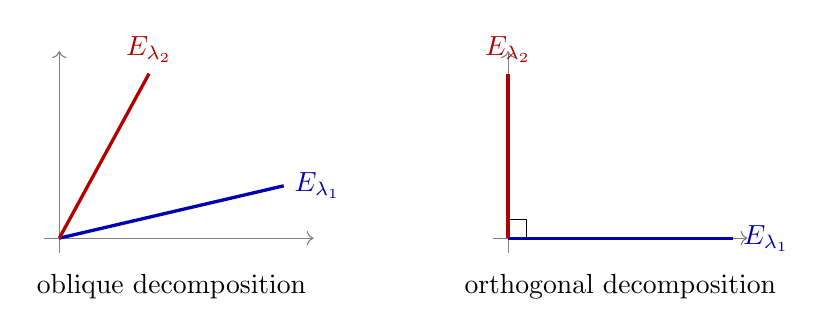
\begin{tikzpicture}[scale=0.95]
  \draw[->,gray] (-0.2,0)--(3.4,0);
  \draw[->,gray] (0,-0.2)--(0,2.5);
  \draw[very thick,blue!70!black] (0,0)--(3,0.7) node[right] {$E_{\lambda_1}$};
  \draw[very thick,red!70!black] (0,0)--(1.2,2.2) node[above] {$E_{\lambda_2}$};
  \node at (1.5,-0.65) {oblique decomposition};

  \begin{scope}[xshift=6cm]
  \draw[->,gray] (-0.2,0)--(3.2,0);
  \draw[->,gray] (0,-0.2)--(0,2.5);
  \draw[very thick,blue!70!black] (0,0)--(3,0) node[right] {$E_{\lambda_1}$};
  \draw[very thick,red!70!black] (0,0)--(0,2.2) node[above] {$E_{\lambda_2}$};
  \draw (0.25,0)--(0.25,0.25)--(0,0.25);
  \node at (1.5,-0.65) {orthogonal decomposition};
  \end{scope}
\end{tikzpicture}
\end{center}

\vfill

\begin{center}
\x{Normal matrices are exactly the matrices whose spectral pieces are orthogonal.}
\end{center}

\end{frame}

\begin{frame}[shrink=5]{The Main Theorem}

\begin{thm}[Normal Matrix Theorem]
For a complex matrix $A$,

$$
A\text{ is normal}
\quad\Longleftrightarrow\quad
\begin{array}{c}
A\text{ is diagonalizable}\\
\text{and distinct eigenspaces are Hermitian-orthogonal.}
\end{array}
$$
\end{thm}

\vfill

In spectral projection language:

$$
A\text{ normal}
\quad\Longleftrightarrow\quad
P_i^H=P_i\quad\text{for all }i.
$$

\vfill

\begin{center}
\x{Diagonalizable is not the endpoint. Orthogonal eigenspaces are the endpoint.}
\end{center}

\end{frame}

% ============================================================
\section{Hermitian Geometry}
% ============================================================

\begin{frame}{Why Complex Geometry Needs Repair}

Over real numbers, length comes from

$$
\|v\|^2=v^Tv.
$$

\vfill

However, problem arises when working over complex numbers.

\vfill

Take

$$
v=\begin{pmatrix}1\\ i\end{pmatrix}.
$$

Then

$$
v^Tv=1+i^2=0.
$$

\vfill

\begin{center}
\x{A nonzero vector should not have length zero.}
\end{center}

\end{frame}

\begin{frame}{The Repair: Conjugate First}

The complex mirror of a vector is

$$
v^H=\overline{v}^{\,T}.
$$

\vfill

For

$$
v=\begin{pmatrix}1\\ i\end{pmatrix},
\qquad
v^H=\begin{pmatrix}1&-i\end{pmatrix}.
$$

\vfill

Now

$$
v^Hv=1+(-i)i=2.
$$

\vfill

\begin{center}
\x{Complex length is Hermitian length.}
\end{center}

\end{frame}

\begin{frame}{Hermitian Inner Product}

\begin{defi}[Hermitian Inner Product]
For $v,w\in\mathbb C^n$, define

$$
\langle v,w\rangle_H=v^Hw.
$$
\end{defi}

\vfill

Then

$$
\langle v,v\rangle_H
=v^Hv
=|v_1|^2+|v_2|^2+\cdots+|v_n|^2\ge0.
$$

\vfill

And

$$
v^Hv=0\quad\Longleftrightarrow\quad v=0.
$$

\end{frame}

\begin{frame}{Hermitian Orthogonality}

\begin{defi}[Hermitian Orthogonal Vectors]
Two vectors $v,w\in\mathbb C^n$ are \x{Hermitian-orthogonal} if

$$
v^Hw=0.
$$

We write

$$
v\perpH w.
$$
\end{defi}

\vfill

\begin{defi}[Hermitian-Orthogonal Subspaces]
Subspaces $V,W\subseteq\mathbb C^n$ satisfy $V\perpH W$ if

$$
v^Hw=0
\quad\text{for every }v\in V,
\quad w\in W.
$$
\end{defi}

\end{frame}

\begin{frame}{Hermitian Direct Sum}

When eigenspaces are Hermitian-orthogonal, we write

$$
\mathbb C^n
=E_{\lambda_1}\orthoplusH E_{\lambda_2}\orthoplusH\cdots\orthoplusH E_{\lambda_k}.
$$

\vfill

This means every vector has a unique decomposition

$$
v=v_1+v_2+\cdots+v_k,
\qquad v_i\in E_{\lambda_i},
$$

and different pieces are perpendicular:

$$
v_i^Hv_j=0\qquad (i\ne j).
$$

\vfill

\begin{center}
\x{This is the geometric meaning of normality.}
\end{center}

\end{frame}

% ============================================================
\section{Hermitian Conjugate and Normality}
% ============================================================

\begin{frame}{Hermitian Conjugate of a Matrix}

\begin{defi}[Hermitian Conjugate]
For a complex matrix $A$, define

$$
A^H=\overline{A}^{\,T}.
$$
\end{defi}

\vfill

Example:

$$
A=\begin{pmatrix}1&i\\2-i&3\end{pmatrix},
\qquad
A^H=\begin{pmatrix}1&2+i\\-i&3\end{pmatrix}.
$$

\vfill

If $A$ is real, then $A^H=A^T$.

\end{frame}

\begin{frame}{Product Rule}

Hermitian conjugate reverses multiplication order:

$$
\boxed{(AB)^H=B^HA^H.}
$$

\vfill

So $H$ behaves like transpose, but with complex conjugation added.

\vfill

\begin{center}
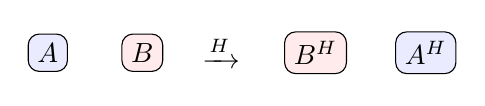
\begin{tikzpicture}
\node[draw,rounded corners,fill=blue!8] (a) at (0,0) {$A$};
\node[draw,rounded corners,fill=red!8] (b) at (1.2,0) {$B$};
\node at (2.2,0) {$\xrightarrow{H}$};
\node[draw,rounded corners,fill=red!8] (bh) at (3.4,0) {$B^H$};
\node[draw,rounded corners,fill=blue!8] (ah) at (4.8,0) {$A^H$};
\end{tikzpicture}
\end{center}

\end{frame}

\begin{frame}{Normal Matrix}

\begin{defi}[Normal Matrix]
A complex square matrix $A$ is \x{normal} if

$$
AA^H=A^HA.
$$
\end{defi}

\vfill

\begin{center}
\x{It means exactly this equation: $A$ commutes with $A^H$.}
\end{center}

\end{frame}

\begin{frame}[shrink=8]{Special Normal Matrices}

\begin{center}
\renewcommand{\arraystretch}{1.25}
\begin{tabular}{c|c|c}
\textbf{Name} & \textbf{Equation} & \textbf{Example}\\
\hline
Hermitian & $A^H=A$ &
$\begin{pmatrix}1&i\\-i&2\end{pmatrix}$\\[0.7em]
Skew-Hermitian & $A^H=-A$ &
$\begin{pmatrix}i&1\\-1&2i\end{pmatrix}$\\[0.7em]
Unitary & $A^HA=I$ &
$\begin{pmatrix}0&1\\1&0\end{pmatrix}$
\end{tabular}
\end{center}

\vfill

\begin{center}
\x{These are not separate topics. They are special normal matrices.}
\end{center}

\end{frame}

\begin{frame}{Non-Example}

Let

$$
J=\begin{pmatrix}1&1\\0&1\end{pmatrix}.
$$

\vfill

Then

$$
JJ^H
=\begin{pmatrix}2&1\\1&1\end{pmatrix},
\qquad
J^HJ
=\begin{pmatrix}1&1\\1&2\end{pmatrix}.
$$

\vfill

So

$$
JJ^H\ne J^HJ.
$$

\vfill

\begin{center}
\x{$J$ is not normal. Its eigen-directions are not orthogonal geometry.}
\end{center}

\end{frame}

% ============================================================
\section{Proof Plan}
% ============================================================

\begin{frame}[shrink=8]{Recall: Radical Criterion}

Write the characteristic polynomial honestly as

$$
\det(tI-A)
=\prod_{i=1}^k(t-\lambda_i)^{m_i}.
$$

\vfill

The radical polynomial removes repeated powers:

$$
r_A(t)=\prod_{i=1}^k(t-\lambda_i).
$$

\vfill

From previous lectures:

\begin{thm}[Radical Criterion for Diagonalizability]
For a complex matrix $A$,

$$
\boxed{
A\text{ diagonalizable}
\quad\Longleftrightarrow\quad
r_A(A)=0.
}
$$
\end{thm}

\vfill

\begin{center}
\x{This is the criterion we are trying to force for normal matrices.}
\end{center}

\end{frame}


\begin{frame}[shrink=8]{Goal and Subgoals}

Goal:

$$
\boxed{A\text{ normal}\quad\Longrightarrow\quad A\text{ diagonalizable}.}
$$

\vfill

By the recalled radical criterion,

$$
A\text{ diagonalizable}
\quad\Longleftrightarrow\quad
r_A(A)=0.
$$

So the proof goal becomes:

$$
\boxed{r_A(A)=0.}
$$

\vfill

\begin{center}
\scriptsize
\renewcommand{\arraystretch}{1.35}
\begin{tabular}{c|c|c}
\textbf{Subgoal} & \textbf{Input assumption} & \textbf{Output}\\
\hline
Theorem A & \x{any complex matrix $A$} & $r_A(A)$ is nilpotent\\
Theorem B & $A$ normal, $p(t)$ any polynomial & $p(A)$ is normal\\
Lemma C & $N$ normal and nilpotent & $N=0$
\end{tabular}
\end{center}

\vfill

\begin{center}
\x{Important boundary: Theorem A is true even if $A$ is not normal.}
\end{center}

\end{frame}


\begin{frame}{How the Subgoals Prove the Goal}

Now specialize to a normal matrix $A$:

$$
\underbrace{r_A(A)\text{ is nilpotent}}_{\text{Theorem A: true for every }A}
\qquad\text{and}\qquad
\underbrace{r_A(A)\text{ is normal}}_{\text{Theorem B: uses normality of }A}.
$$

\vfill

Then

$$
\underbrace{r_A(A)=0}_{\text{Lemma C}}.
$$

\vfill

From the previous diagonalization criterion:

$$
r_A(A)=0
\quad\Longrightarrow\quad
A\text{ is diagonalizable}.
$$

\vfill

\begin{center}
\x{After diagonalizability, spectral projections will prove orthogonality.}
\end{center}

\end{frame}

\begin{frame}{Theorem A: $r_A(A)$ Is Nilpotent}

\begin{thm}[Radical Polynomial Produces Nilpotent Matrix]
For every complex matrix $A$, the matrix $r_A(A)$ is nilpotent.
\end{thm}

\vfill

Let

$$
M=\max\{m_1,\ldots,m_k\}.
$$

Then

$$
r_A(t)^M
=\prod_{i=1}^k(t-\lambda_i)^M
=\det(tI-A)q(t).
$$

\vfill

Plug in $A$:

$$
r_A(A)^M=0.
$$

\end{frame}

\begin{frame}{Theorem B: Polynomials Preserve Normality}

\begin{thm}[Polynomial of a Normal Matrix]
If $A$ is normal, then every polynomial $p(A)$ is normal.
\end{thm}

\vfill

Normality says

$$
AA^H=A^HA.
$$

\vfill

So every power of $A$ commutes with every power of $A^H$:

$$
A^m(A^H)^n=(A^H)^nA^m.
$$

\vfill

Therefore $p(A)$ commutes with $p(A)^H$.

\end{frame}

\begin{frame}{Positivity Lemma for Matrices}

\begin{lem}[Matrix Positivity]
If $MM^H=0$, then $M=0$.
\end{lem}

\vfill

List the rows of $M$ as

$$
M=
\begin{pmatrix}
-&r_1^H&-\\
-&r_2^H&-\\
 &\vdots& \\
-&r_m^H&-
\end{pmatrix}.
$$

\vfill

Then $MM^H$ is the inner-product table of the rows.

\end{frame}


\begin{frame}{Positivity Lemma: Inner-Product Table}

\[
\underbrace{
\begin{pmatrix}
-&r_1^H&-\\
-&r_2^H&-\\
 &\vdots& \\
-&r_m^H&-
\end{pmatrix}}_{M}
\underbrace{
\begin{pmatrix}
|&|&&|\\
r_1&r_2&\cdots&r_m\\
|&|&&|
\end{pmatrix}}_{M^H}
=
\underbrace{
\begin{pmatrix}
r_1^Hr_1&r_1^Hr_2&\cdots&r_1^Hr_m\\
r_2^Hr_1&r_2^Hr_2&\cdots&r_2^Hr_m\\
\vdots&\vdots&\ddots&\vdots\\
r_m^Hr_1&r_m^Hr_2&\cdots&r_m^Hr_m
\end{pmatrix}}_{MM^H}.
\]

\vfill

If $MM^H=0$, then in particular every diagonal entry is zero:

$$
r_i^Hr_i=0\quad\Longrightarrow\quad r_i=0.
$$

\vfill

So every row is zero, hence $M=0$.

\end{frame}


\begin{frame}{Lemma C: Normal Nilpotent Collapse}

\begin{lem}[Normal Nilpotent Matrices Vanish]
If $N$ is normal and nilpotent, then

$$
N=0.
$$
\end{lem}

\vfill

This is where the matrix positivity lemma enters:

$$
MM^H=0\quad\Longrightarrow\quad M=0.
$$

\vfill

We prove this by descending from a high zero power down to $N=0$.

\end{frame}

\begin{frame}[shrink=10]{Lemma C: Descent Step}

Assume

$$
N^{2^r}=0.
$$

\vfill

Since $N$ is normal, $N$ commutes with $N^H$.

\vfill

Then write the power as repeated factors:

$$
0=
\underbrace{NN\cdots N}_{2^r\text{ many}}
\underbrace{N^HN^H\cdots N^H}_{2^r\text{ many}}.
$$

\vfill

Because $N$ commutes with $N^H$, regroup this as:

$$
0=
\underbrace{
\left(
\underbrace{NN\cdots N}_{2^{r-1}\text{ many}}
\underbrace{N^HN^H\cdots N^H}_{2^{r-1}\text{ many}}
\right)}_{M}
\underbrace{
\left(
\underbrace{NN\cdots N}_{2^{r-1}\text{ many}}
\underbrace{N^HN^H\cdots N^H}_{2^{r-1}\text{ many}}
\right)^H}_{M^H}.
$$

\vfill

By the matrix positivity lemma,

$$
N^{2^{r-1}}(N^H)^{2^{r-1}}=0.
$$

\end{frame}

\begin{frame}{Lemma C: Finish}

Repeat the descent:

$$
N^{2^r}=0
\Rightarrow
N^{2^{r-1}}(N^H)^{2^{r-1}}=0
\Rightarrow\cdots\Rightarrow
NN^H=0.
$$

\vfill

By positivity again:

$$
NN^H=0\quad\Longrightarrow\quad N=0.
$$

\vfill

\begin{center}
\x{Normal plus nilpotent leaves no room except zero.}
\end{center}

\end{frame}

\begin{frame}{Normal Implies Diagonalizable}

For normal $A$:

\begin{itemize}
\item Theorem A: $r_A(A)$ is nilpotent.
\item Theorem B: $r_A(A)$ is normal.
\item Lemma C: normal nilpotent matrices vanish.
\end{itemize}

\vfill

Therefore

$$
r_A(A)=0.
$$

\vfill

By the radical criterion:

$$
\boxed{A\text{ is diagonalizable}.}
$$

\vfill

\begin{center}
\x{But this is only the checkpoint, not the endpoint.}
\end{center}

\end{frame}

% ============================================================
\section{Spectral Projections}
% ============================================================

\begin{frame}{Spectral Projections Return}

For a diagonalizable matrix with distinct eigenvalues $\lambda_i$, previous lectures gave

$$
P_i=f_i(A),
$$

where $f_i$ is the Lagrange interpolation polynomial satisfying

$$
f_i(\lambda_j)=\delta_{ij}.
$$

\vfill

Then

$$
I=P_1+\cdots+P_k,
\qquad
P_iP_j=0\ (i\ne j),
\qquad
A=\sum_i\lambda_iP_i.
$$

\end{frame}

\begin{frame}{What Does $P_i$ Do?}

The projection $P_i$ extracts the $\lambda_i$-eigenspace component:

$$
\operatorname{Im}(P_i)=E_{\lambda_i}.
$$

\vfill

Every vector decomposes as

$$
v=P_1v+P_2v+\cdots+P_kv.
$$

\vfill

Question:

$$
\boxed{\text{Are these projections oblique or Hermitian-orthogonal?}}
$$

\vfill

\begin{center}
\x{For normal matrices, they are Hermitian-orthogonal projections.}
\end{center}

\end{frame}

\begin{frame}{Normality Passes to Spectral Projections}

If $A$ is normal, then by Theorem B every polynomial in $A$ is normal.

\vfill

But

$$
P_i=f_i(A).
$$

\vfill

Therefore

$$
\boxed{P_i\text{ is normal}.}
$$

\vfill

Also, by construction,

$$
P_i^2=P_i.
$$

\vfill

\begin{center}
\x{So each spectral projection is a normal projection.}
\end{center}

\end{frame}

\begin{frame}{The Central Lemma}

\begin{lem}[Normal Projection Is Hermitian]
If

$$
P^2=P
\qquad\text{and}\qquad
PP^H=P^HP,
$$

then

$$
P=P^H.
$$
\end{lem}

\vfill

\begin{center}
\x{Normality kills obliqueness for projections.}
\end{center}

\end{frame}

\begin{frame}{Proof: Algebra Setup}

We prove $P=P^H$ by proving

$$
P-PP^H=0.
$$

\vfill

Let

$$
M=P-PP^H.
$$

\vfill

By the matrix positivity lemma, it is enough to show

$$
MM^H=0.
$$

\vfill

\begin{center}
\x{Everything now is algebra: expand and simplify.}
\end{center}

\end{frame}


\begin{frame}{Proof: Expand $MM^H$}

Since $(PP^H)^H=PP^H$,

$$
M^H=P^H-PP^H.
$$

\vfill

So

$$
\begin{aligned}
MM^H
&=(P-PP^H)(P^H-PP^H)\\
&=PP^H-P(PP^H)-(PP^H)P^H+(PP^H)(PP^H).
\end{aligned}
$$

\vfill

\begin{center}
\x{Now use $P^2=P$, $(P^H)^2=P^H$, and $PP^H=P^HP$.}
\end{center}

\end{frame}


\begin{frame}{Proof: Simplify}

Term by term:

$$
P(PP^H)=P^2P^H=PP^H.
$$

\vfill

$$
(PP^H)P^H=P(P^H)^2=PP^H.
$$

\vfill

For the last term:

$$
(PP^H)(PP^H)
=P(P^HP)P^H
=P(PP^H)P^H
=P^2(P^H)^2
=PP^H.
$$

\end{frame}


\begin{frame}{Proof: Finish}

Substitute these into the expansion:

$$
MM^H
=PP^H-PP^H-PP^H+PP^H=0.
$$

\vfill

By the matrix positivity lemma:

$$
MM^H=0\quad\Longrightarrow\quad M=0.
$$

\vfill

So

$$
P-PP^H=0,
\qquad\text{hence}\qquad
P=PP^H.
$$

\vfill

Taking $H$ gives $P^H=PP^H$, so $P=P^H$.

\end{frame}


\begin{frame}{Projection Payoff}

Every spectral projection of a normal matrix satisfies

$$
P_i^2=P_i,
\qquad
P_iP_i^H=P_i^HP_i.
$$

\vfill

By the central lemma:

$$
P_i=P_i^H.
$$

\vfill

\begin{center}
\x{This is where orthogonal eigenspaces come from.}
\end{center}

\end{frame}


\begin{frame}{Main Payoff}

For normal $A$:

\begin{itemize}
\item $A$ is diagonalizable.
\item $P_i=f_i(A)$ are spectral projections.
\item $P_i$ are normal because polynomials preserve normality.
\item $P_i^2=P_i$ because they are projections.
\item Therefore $P_i=P_i^H$.
\end{itemize}

\vfill

So every spectral projection is Hermitian symmetric.

\end{frame}

\begin{frame}{Orthogonal Eigenspaces}

If $P_i=P_i^H$, then $P_i$ is an orthogonal projection.

\vfill

For $i\ne j$,

$$
P_iP_j=0.
$$

\vfill

Take $v\in E_{\lambda_i}=\operatorname{Im}(P_i)$ and $w\in E_{\lambda_j}=\operatorname{Im}(P_j)$.

Then

$$
v^Hw
=(P_iv)^H(P_jw)
=v^HP_i^HP_jw
=v^HP_iP_jw=0.
$$

\vfill

\begin{center}
\x{Distinct eigenspaces are Hermitian-orthogonal.}
\end{center}

\end{frame}

\begin{frame}{Converse Direction}

Assume $A$ is diagonalizable and all spectral projections are Hermitian:

$$
A=\sum_i\lambda_iP_i,
\qquad
P_i^H=P_i,
\qquad
P_iP_j=0\ (i\ne j).
$$

\vfill

Then

$$
A^H=\sum_i\overline{\lambda_i}P_i.
$$

\vfill

So

$$
AA^H=\sum_i|\lambda_i|^2P_i
=A^HA.
$$

\vfill

Therefore $A$ is normal.

\end{frame}

\begin{frame}{Main Theorem, Proven}

\begin{thm}[Normal Matrix Theorem]
For a complex matrix $A$,

$$
A\text{ normal}
\quad\Longleftrightarrow\quad
\begin{array}{c}
A\text{ is diagonalizable}\\
\text{and distinct eigenspaces are Hermitian-orthogonal.}
\end{array}
$$
\end{thm}

\vfill

Equivalently:

$$
\boxed{
A\text{ normal}
\quad\Longleftrightarrow\quad
P_i=P_i^H\text{ for all }i.
}
$$

\end{frame}

% ============================================================
\section{Unitary Diagonalization}
% ============================================================

\begin{frame}{Collect Orthonormal Eigenvectors}

Because eigenspaces are Hermitian-orthogonal, we can choose an orthonormal basis inside each eigenspace and stack all of them:

$$
\Omega=\begin{pmatrix}|&|&&|\\
u_1&u_2&\cdots&u_n\\
|&|&&|
\end{pmatrix}.
$$

\vfill

Then

$$
\Omega^H\Omega=I.
$$

\vfill

So $\Omega$ is unitary.

\end{frame}

\begin{frame}{Unitary Diagonalization}

With the orthonormal eigenbasis matrix $\Omega$,

$$
A\Omega=\Omega\Lambda.
$$

\vfill

Multiply by $\Omega^H$:

$$
\boxed{\Omega^HA\Omega=\Lambda.}
$$

\vfill

Equivalently,

$$
\boxed{A=\Omega\Lambda\Omega^H.}
$$

\vfill

\begin{center}
\x{Unitary diagonalization is a consequence of orthogonal eigenspaces.}
\end{center}

\end{frame}


% ============================================================
\section{Complete Example}
% ============================================================

\begin{frame}{Example: Start from a Hermitian Matrix}

Let

\[
\underbrace{
\begin{pmatrix}
-2&1&1\\
1&-2&1\\
1&1&-2
\end{pmatrix}}_{A}.
\]

\vfill

This matrix is Hermitian symmetric:

$$
A^H=A.
$$

\vfill

Therefore:

$$
A\text{ Hermitian}
\Longrightarrow
A\text{ normal}
\Longrightarrow
A\text{ diagonalizable}.
$$

\end{frame}


\begin{frame}{Example: Radical Criterion}

Compute the characteristic polynomial:

$$
\det(tI-A)=t(t+3)^2.
$$

\vfill

So the radical polynomial is

$$
r_A(t)=t(t+3).
$$

\vfill

Since $A$ is normal, it is diagonalizable.  Therefore the radical criterion gives:

$$
\boxed{r_A(A)=A(A+3I)=0.}
$$

\vfill

\begin{center}
\x{Now we can use the spectral-projection recipe from previous lectures.}
\end{center}

\end{frame}


\begin{frame}{Example: Polynomial Remainder Formula}

For any polynomial $g(t)$, reduce $g$ modulo

$$
r_A(t)=t(t+3).
$$

\vfill

The two eigenvalues are $0$ and $-3$.

\vfill

By Lagrange interpolation:

$$
g(A)
=
g(0)\underbrace{\frac{A+3I}{3}}_{P_0}
+
g(-3)\underbrace{\frac{-A}{3}}_{P_{-3}}.
$$

\vfill

So the spectral projections are:

$$
\boxed{P_0=\frac{A+3I}{3}},
\qquad
\boxed{P_{-3}=\frac{-A}{3}}.
$$

\end{frame}


\begin{frame}{Example: Honest Projection Matrices}

\[
P_0
=
\frac13
\left(
\underbrace{
\begin{pmatrix}
-2&1&1\\
1&-2&1\\
1&1&-2
\end{pmatrix}}_{A}
+3I
\right)
=
\underbrace{
\frac13
\begin{pmatrix}
1&1&1\\
1&1&1\\
1&1&1
\end{pmatrix}}_{P_0}.
\]

\vfill

\[
P_{-3}
=
\underbrace{
I-P_0
}_{P_{-3}}
=
\underbrace{
\frac13
\begin{pmatrix}
2&-1&-1\\
-1&2&-1\\
-1&-1&2
\end{pmatrix}}_{P_{-3}}.
\]

\end{frame}


\begin{frame}{Example: Projection Decomposition}

The spectral decomposition is:

\[
\underbrace{
\begin{pmatrix}
-2&1&1\\
1&-2&1\\
1&1&-2
\end{pmatrix}}_{A}
=
0\cdot
\underbrace{
\frac13
\begin{pmatrix}
1&1&1\\
1&1&1\\
1&1&1
\end{pmatrix}}_{P_0}
-3\cdot
\underbrace{
\frac13
\begin{pmatrix}
2&-1&-1\\
-1&2&-1\\
-1&-1&2
\end{pmatrix}}_{P_{-3}}.
\]

\vfill

\begin{center}
\x{The projections are Hermitian, so their column spaces are orthogonal.}
\end{center}

\end{frame}


\begin{frame}{Example: Diagonal Cross-Fill $P_0$}

The projection $P_0$ is rank one:

\[
P_0=
\frac13
\begin{pmatrix}
1&1&1\\
1&1&1\\
1&1&1
\end{pmatrix}
=
\underbrace{
\begin{pmatrix}
\frac1{\sqrt3}\\[0.2em]
\frac1{\sqrt3}\\[0.2em]
\frac1{\sqrt3}
\end{pmatrix}
\begin{pmatrix}
\frac1{\sqrt3}&\frac1{\sqrt3}&\frac1{\sqrt3}
\end{pmatrix}}_{u_1u_1^H}.
\]

\vfill

So one unit eigenvector for eigenvalue $0$ is

$$
u_1=\frac1{\sqrt3}\begin{pmatrix}1\\1\\1\end{pmatrix}.
$$

\end{frame}


\begin{frame}[shrink=16]{Example: Diagonal Cross-Fill $P_{-3}$}

Now cross-fill the orthogonal projection $P_{-3}$.

\[
\underbrace{
\frac13
\begin{pmatrix}
2&-1&-1\\
-1&2&-1\\
-1&-1&2
\end{pmatrix}}_{P_{-3}}
=
\underbrace{
\begin{pmatrix}
\sqrt{\frac23}\\[0.2em]
-\frac1{\sqrt6}\\[0.2em]
-\frac1{\sqrt6}
\end{pmatrix}
\begin{pmatrix}
\sqrt{\frac23}&-\frac1{\sqrt6}&-\frac1{\sqrt6}
\end{pmatrix}}_{u_2u_2^H}
+
\underbrace{
\begin{pmatrix}
0\\[0.2em]
\frac1{\sqrt2}\\[0.2em]
-\frac1{\sqrt2}
\end{pmatrix}
\begin{pmatrix}
0&\frac1{\sqrt2}&-\frac1{\sqrt2}
\end{pmatrix}}_{u_3u_3^H}.
\]

\end{frame}


\begin{frame}[shrink=15]{Example: One Equality Chain}

The diagonalization is not a separate trick.
It is the same spectral decomposition, after cross-filling the projections:

\[
\scriptsize
\begin{aligned}
\underbrace{
\begin{pmatrix}
-2&1&1\\
1&-2&1\\
1&1&-2
\end{pmatrix}}_{A}
&=
\bl{0}\underbrace{\bl{u_1}\bl{u_1^H}}_{\bl{P_0}}
\ora{(-3)}\underbrace{\ora{u_2}\ora{u_2^H}}_{\ora{\text{rank-one part of }P_{-3}}}
\gn{(-3)}\underbrace{\gn{u_3}\gn{u_3^H}}_{\gn{\text{rank-one part of }P_{-3}}}
\\[0.7em]
&=
\underbrace{
\begin{pmatrix}
|&|&|\\
\bl{u_1}&\ora{u_2}&\gn{u_3}\\
|&|&|
\end{pmatrix}}_{\Omega}
\underbrace{
\begin{pmatrix}
\bl{0}&0&0\\
0&\ora{-3}&0\\
0&0&\gn{-3}
\end{pmatrix}}_{\Lambda}
\underbrace{
\begin{pmatrix}
-&\bl{u_1^H}&-\\
-&\ora{u_2^H}&-\\
-&\gn{u_3^H}&-
\end{pmatrix}}_{\Omega^H}
\\[0.7em]
&=
\boxed{\Omega\Lambda\Omega^H}.
\end{aligned}
\]

\[
\Omega=
\begin{pmatrix}
\frac1{\sqrt3}&\sqrt{\frac23}&0\\[0.25em]
\frac1{\sqrt3}&-\frac1{\sqrt6}&\frac1{\sqrt2}\\[0.25em]
\frac1{\sqrt3}&-\frac1{\sqrt6}&-\frac1{\sqrt2}
\end{pmatrix},
\qquad
\Omega^H\Omega=I.
\]

\end{frame}


% ============================================================
\section*{Special Normal Matrices}
% ============================================================

\begin{frame}{Eigenvalue Geometry}

For a normal matrix,

$$
A=\sum_i\lambda_iP_i,
\qquad
P_i=P_i^H.
$$

\vfill

Then

$$
A^H=\sum_i\overline{\lambda_i}P_i.
$$

\vfill

So any extra equation involving $A^H$ becomes an equation about eigenvalues.

\vfill

\begin{center}
\x{Special normal matrices are eigenvalue-location restrictions.}
\end{center}

\end{frame}

\begin{frame}[shrink=8]{Hermitian Matrices}

Suppose

$$
A^H=A.
$$

\vfill

Compare spectral decompositions:

$$
\sum_i\overline{\lambda_i}P_i
=
\sum_i\lambda_iP_i.
$$

\vfill

Therefore

$$
\overline{\lambda_i}=\lambda_i.
$$

\vfill

So

$$
\boxed{\lambda_i\in\mathbb R.}
$$

\vfill

\begin{center}
\x{Hermitian means: eigenvalues lie on the real axis.}
\end{center}

\end{frame}

\begin{frame}[shrink=8]{Skew-Hermitian Matrices}

Suppose

$$
A^H=-A.
$$

\vfill

Compare spectral decompositions:

$$
\sum_i\overline{\lambda_i}P_i
=
-
\sum_i\lambda_iP_i.
$$

\vfill

Therefore

$$
\overline{\lambda_i}=-\lambda_i.
$$

\vfill

So

$$
\boxed{\lambda_i\in i\mathbb R.}
$$

\vfill

\begin{center}
\x{Skew-Hermitian means: eigenvalues lie on the imaginary axis.}
\end{center}

\end{frame}

\begin{frame}[shrink=8]{Unitary Matrices}

Suppose

$$
A^HA=I.
$$

\vfill

Using

$$
A=\sum_i\lambda_iP_i,
\qquad
A^H=\sum_i\overline{\lambda_i}P_i,
$$

we get

$$
A^HA=\sum_i|\lambda_i|^2P_i.
$$

\vfill

Thus

$$
|\lambda_i|^2=1.
$$

\vfill

\begin{center}
\x{Unitary means: eigenvalues lie on the unit circle.}
\end{center}

\end{frame}

\begin{frame}[shrink=8]{Complex Plane Summary}

\begin{center}
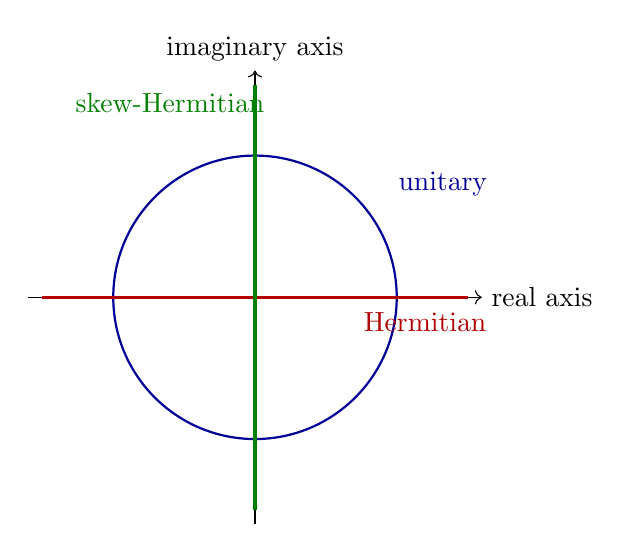
\begin{tikzpicture}[scale=0.9]
  \draw[->] (-3.2,0)--(3.2,0) node[right] {real axis};
  \draw[->] (0,-3.2)--(0,3.2) node[above] {imaginary axis};
  \draw[thick,blue!60!black] (0,0) circle (2);
  \node[blue!60!black] at (2.65,1.6) {unitary};
  \node[red!70!black] at (2.4,-0.35) {Hermitian};
  \node[green!50!black] at (-1.2,2.75) {skew-Hermitian};
  \draw[very thick,red!70!black] (-3,0)--(3,0);
  \draw[very thick,green!50!black] (0,-3)--(0,3);
\end{tikzpicture}
\end{center}

\vfill

\begin{center}
\renewcommand{\arraystretch}{1.25}
\begin{tabular}{c|c}
\textbf{Matrix type} & \textbf{Eigenvalue location}\\
\hline
Hermitian & real axis\\
Skew-Hermitian & imaginary axis\\
Unitary & unit circle
\end{tabular}
\end{center}

\end{frame}

\begin{frame}{Final Summary}

The core theorem is:

$$
\boxed{AA^H=A^HA}
\quad\Longleftrightarrow\quad
\boxed{P_i=P_i^H\text{ for all }i.}
$$

$$
\Longleftrightarrow
\boxed{E_{\lambda_i}\perpH E_{\lambda_j}\quad(i\ne j).}
$$

\vfill

Special normal matrices add eigenvalue restrictions:

$$
\begin{array}{ccl}
A^H=A &\Longleftrightarrow& \lambda_i\in\mathbb R,\\[0.3em]
A^H=-A &\Longleftrightarrow& \lambda_i\in i\mathbb R,\\[0.3em]
A^HA=I &\Longleftrightarrow& |\lambda_i|=1.
\end{array}
$$

\vfill

\begin{center}
\x{Normal matrices turn spectral decomposition into orthogonal geometry.}
\end{center}

\end{frame}

\end{document}
